\documentclass[letterpaper,12pt,fleqn]{article}
\usepackage{matharticle}
\usepackage{tikz}
\usetikzlibrary{decorations.markings}
\usetikzlibrary{shapes}
\pagestyle{empty}
\newcommand{\T}{\mathscr{T}}
\renewcommand{\a}{\alpha}
\renewcommand{\l}{\lambda}
\renewcommand{\O}{\theta}
\begin{document}
\section*{Quotient Maps}

New spaces can be created from existing spaces by identifying (gluing) points in new spaces via equivalence
relations.

\begin{example}[Cylinder]

  Identifying two edges of a square to make a cylinder:

  \bigskip

  \begin{minipage}{3in}
    \centering
    \begin{tikzpicture}
      \begin{scope}[decoration={markings,mark=at position 0.5 with {\arrow[scale=4]{>}}}]
        \draw [postaction={decorate}] (0,0) -- (4,0);
        \draw [postaction={decorate}] (0,4) -- (4,4);
      \end{scope}
      \draw (0,0) -- (0,4);
      \draw (4,0) -- (4,4);
    \end{tikzpicture}

    \bigskip

    \(X=[0,1]\times[0,1]\)
  \end{minipage}
  \begin{minipage}{3in}
    \centering
    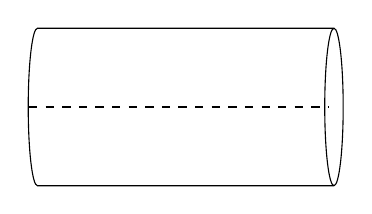
\begin{tikzpicture}
      \node [draw,cylinder,minimum width=2cm,minimum height=4cm] at (0,0) {};
      \draw [dashed] (-1.9,0) -- (1.9,0);
    \end{tikzpicture}

    \bigskip

    \(C\)
  \end{minipage}

  The gluing function \(g:X\to C\) defined by:
  \[g(x,y)=(x,\sin(2\pi y),\cos(2\pi y))\]
  A set is \(U\) is open in \(C\) iff \(g^{-1}(U)\) is open in \(X\).  Thus, gluing functions are automatically
  continuous.

  However, it is easier to identify points using equivalence relations that partition the identified points.
  \[C=\setb{\set{(x,y)}}{x\in[0,1],y\in(0,1)}\cup\setb{\set{(x,0),(x,1)}}{x\in[0,1]}\]
\end{example}

\begin{definition}[Identification Space]
  Let \(X\) be a topological space and let \(\sim\) be an equivalence relation on \(X\).  The function
  \(f:X\to X/\sim\) defined by \(f(X)=X/\sim\) is called an \emph{identification map}.  The resulting space \(X^*\)
  of equivalence classes is called an \emph{identification space}.  A set \(U\) is open in \(X^*\) iff \(f^{-1}(U)\)
  is open in \(X\).  Hence, \(f\) is continuous by definition.
\end{definition}

\begin{example}[M\"{o}bius Band]
  Construct a M\"{o}bius band explicitly as an identification space of \(X=[0,8]\times[0,1]\).
  \[X^*=\setb{\set{(x,y)}}{x\in(0,8),y\in[0,1]}\cup\setb{{(0,y),(8,1-y)}}{y\in[0,1]}\]
\end{example}

\begin{example}[Torus]
  Construct a torus explicitly as:
  \begin{enumerate}
  \item An identification space of a cylinder \(C\).
    \[C=\setb{(R\sin\O,R\cos\O,\ell)}{\O\in[0,2\pi),\ell\in[0,L]}\]
    \begin{align*}
      C^* =& \setb{\set{(R\sin\O,R\cos\O,\ell)}}{\O\in[0,2\pi),\ell\in(0,L)}\cup \\
      & \setb{\set{(R\sin\O,R\cos\O,0),(R\sin\O,R\cos\O,L)}}{\O\in[0,2\pi)}
    \end{align*}
  \item An identification space of \(X=[0,1]\times[0,1]\).
    \begin{align*}
      X^* =& \setb{\set{(x,y)}}{x\in(0,1),y\in(0,1)}\cup \\
      & \setb{\set{(x,0),(x,1)}}{x\in(0,1)}\cup \\
      & \setb{\set{(0,y),(1,y)}}{y\in[0,1]}
    \end{align*}
  \item An identification space of \(\R^2\).
    \[(x,y)\sim(u,v)\iff x-u\in\Z\ \text{and}\ y-v\in\Z\]
  \end{enumerate}
\end{example}

\begin{definition}[Quotient Topology]
  Let \(X\) be a topological space and \(Y\) be a set, and let \(f:X\to Y\) be surjective.  The
  \emph{quotient topology} on \(Y\) with respect to \(f\) is the collection of all \(U\subset Y\) such that
  \(f^{-1}(U)\in\T_X\).  Thus, \(f\) is continuous by definition.
\end{definition}

\begin{theorem}
  The quotient topology actually defines a topology.
\end{theorem}

\begin{proof}
  Assume \(X\) is a topological space, \(Y\) is a set, and \(f:X\to Y\) is surjective.
  \begin{enumerate}
  \item \(f^{-1}(\emptyset)=\emptyset\in\T_X\).  Therefore \(\emptyset\in\T_Y\).

  \item \(f^{-1}(Y)=X\in\T_X\).  Therefore \(Y\in\T_Y\).

  \item Assume that \(U,V\in\T_Y\).  This means that \(f^{-1}(U),f^{-1}(V)\in\T_X\) and so:
    \[f^{-1}(U)\cap f^{-1}(V)=f^{-1}(U\cap V)\in\T_X\]
    Therefore \(U\cap V\in\T_Y\).

  \item Assume that \(\set{U_{\a}:\a\in\l}\subset\T_Y\).  This means that for all \(a\in\l\),
    \(f^{-1}(U_{\a})\in\T_X\) and so:
    \[\bigcup_{\a\in\l}f^{-1}(U_{\a})=f^{-1}(\bigcup_{\a\in\l}U_{\a})\in\T_X\]
    Therefore \(\bigcup_{\a\in\l}U_{\a}\in\T_Y\).
  \end{enumerate}

  Therefore, the quotient topology on \(Y\) defines a topology.
\end{proof}

\begin{theorem}
  Let \(X\) be a topological space and \(Y\) be a set, and let \(f:X\to Y\) be surjective.  The quotient topology on
  \(Y\) is the finest topology that makes \(f\) continuous.
\end{theorem}

\begin{proof}
  ABC there exists some topology \(\T\) on \(T\) that is finer than \(T_Y\).  Thus, there exists \(U\in\T\) but
  \(U\notin\T_Y\).  This would mean that \(f^{-1}(U)\) is not open in \(X\), contradicting the continuity of \(f\).

  Therefore \(\T=\T_Y\).
\end{proof}

\begin{theorem}
  Let \(X\) and \(Y\) be topological spaces and let \(f:X\to Y\) be a continuous, surjective, open map.  \(f\) is
  a quotient map.
\end{theorem}

\begin{proof}
  Let \(\T_Y^f=\setb{U\subset Y}{f^{-1}(U)\in\T_X}\).  Since \(\T_Y^f\) is the finest topology that makes \(f\)
  continuous, it must be the case that \(\T_Y\subset\T_Y^f\).

  WTS: \(\T_Y^f\subset\T_Y\).

  Assume \(U\in\T_Y^f\).  Then, by definition, \(f^{-1}(U)\in\T_X\).  But \(f\) is open and surjective, so:
  \[f(f^{-1}(U))=U\in\T_Y\]
  Therefore \(\T_Y^f\subset\T_Y\) and hence \(T_Y^f=T_Y\).
\end{proof}

\begin{theorem}
  Let \(X\), \(Y\), and \(Z\) be topological spaces and let \(f:X\to Y\) be a quotient map.  The map \(g:Y\to Z\)
  is continuous iff \(g\circ f\) is continuous.
\end{theorem}

\begin{proof}
  \begin{description}
  \item[]
  \item[\(\implies\)] Assume \(g:Y\to Z\) is continuous.

    But the composition of continuous functions is continuous.

    Therefore \(g\circ f\) is continuous.

  \item[\(\impliedby\)] Assume \(g\circ f\) is continuous.

    Assume \(W\in\T_Z\), and thus \((g\circ f)^{-1}(W)=f^{-1}(g^{-1}(W))\in\T_X\).  But \(f\) is a quotient map, and
    so by definition, \(g^{-1}(W)\in\T_Y\).

    Therefore \(g\) is continuous.
  \end{description}
\end{proof}

\begin{example}
  Quotient maps do not preserve Hausdorff.  As a counterexample, consider \(X=\R^+\times\set{0,1}\) and the
  equivalence relationship \((x,0)\sim(x,1)\).  This yields \(R_{+00}\), which is not Hausdorff.
\end{example}

\end{document}
